\documentclass[12pt]{article}

\usepackage{amssymb,amsmath,amsfonts,bbm,eurosym,geometry,ulem,graphicx,caption,color,setspace,sectsty,comment,footmisc,caption,natbib,pdflscape,subfigure,array,hyperref}


\usepackage{algorithm, algorithmicx}
\usepackage{algpseudocode}
\usepackage{float}
\usepackage{appendix}

\normalem

\onehalfspacing
\newtheorem{theorem}{Theorem}
\newtheorem{corollary}[theorem]{Corollary}
\newtheorem{proposition}{Proposition}
\newenvironment{proof}[1][Proof]{\noindent\textbf{#1.} }{\ \rule{0.5em}{0.5em}}

\newtheorem{hyp}{Hypothesis}
\newtheorem{subhyp}{Hypothesis}[hyp]
\renewcommand{\thesubhyp}{\thehyp\alph{subhyp}}

\newcommand{\red}[1]{{\color{red} #1}}
\newcommand{\blue}[1]{{\color{blue} #1}}
\newcommand{\indep}{\perp \!\!\! \perp}

\newcolumntype{L}[1]{>{\raggedright\let\newline\\arraybackslash\hspace{0pt}}m{#1}}
\newcolumntype{C}[1]{>{\centering\let\newline\\arraybackslash\hspace{0pt}}m{#1}}
\newcolumntype{R}[1]{>{\raggedleft\let\newline\\arraybackslash\hspace{0pt}}m{#1}}
\DeclareMathOperator*{\argmin}{argmin}
\DeclareMathOperator*{\argmax}{argmax}


\geometry{left=1.0in,right=1.0in,top=1.0in,bottom=1.0in}

\begin{document}

\begin{titlepage}
\title{Bayes Optimal Informer Sets for Drug Discovery\thanks{abc}}
\author{Peng Yu, {\sc contributing members of UW drug discovery group}, \\  \& Michael A. Newton\thanks{abc}}
\date{\today}
\maketitle
\begin{abstract}
\noindent Placeholder\\
\vspace{0in}\\
\noindent\textbf{Keywords:} key1, key2, key3\\
\vspace{0in}\\
\noindent\textbf{JEL Codes:} key1, key2, key3\\

\bigskip
\end{abstract}
\setcounter{page}{0}
\thispagestyle{empty}
\end{titlepage}
\pagebreak \newpage




\doublespacing


\section{Background} \label{sec:background}

Zhang, Ericksen, and Lee {\em et al.} (2019) (hereafter, ZEL) introduced
informer-based-ranking (IBR) strategies for computational
guidance of drug-discovery experiments.  The context is 
virtual screening (Sliwoski {\em et al.} 2014).   Briefly, a chemical screening facility receives 
material representing a purified protein target, and is tasked with identifying drugs
that may have some inhibitory effect on the bioactivity of the protein.  For example, ZEL report
on drugs that affect certain protein kinases.
The facility has specific biochemical assays that test for
inhibitory effects of a given drug, and it has access to a very large library of different drug compounds, some small fraction of which are expected to have bioactivity
against the new target.   
Costs limit the number of compounds that may be screened experimentally.   The virtual screening task is to prioritize the drugs 
in advance of experimental screening by some computations so as to
improve the hit rate of the experiments performed on the new target.

Virtual screening may operate on different kinds of target and compound data, including
possibly chemical structures or the results of experimental assays.   For example, when chemical structures are available
it is possible to use sophisticated molecular docking programs that aim to find best fits between target and compound
structures (e.g. cite papers, including our own consensus docking paper.)
We focus on IBR strategies that have access to data on the bioactivity of many compounds
against many targets, though possibly not any bioactivity data from 
the new target on test. **note...no compound structure data is needed**  With these initial bioactivity data, IBR  
identifies a subset of compounds -- the {\em informer set} -- which
represent a small fraction of the available compounds and which we
will test experimentally for bioactivity against the new target.  Subsequently, we use the full set of data (initial data on other targets
for many compounds and intermediate data on informer compounds on 
the new target) in order to prioritize the remaining, non-informer
compounds for their likely bioactivity against the new target.  If
we have done a good job in building the informer set, then the 
top of the prioritized list of non-informers will be enriched
for truly active compounds.  We will have spent computational time
building the informer set from initial data, and experimental resources
obtaining intermediate data; the payoff is that further experiments
will return truly active drug compounds at  a higher rate than
if we had selected compounds to test by some other scheme.

ZEL introduced several bioactivity-based IBR strategies and compared
them empirically in data on protein kinases. Though differing in detail,
the proposed strategies all partition the initial
bioactivity data, producing  clusters of relatively similar targets; 
then informer compounds are  those that are predictive of the cluster label of a target.  Among kinase targets, the proposed bioactivity-based strategies had better predictive
performance than commonly used strategies based upon chemical
structure.   Since effective IBR strategies leverage statistical
patterns in the initial bioactivity data, we reason that
statistical modeling may provide a useful approach to deriving
more effective IBR strategies than are currently available. 
In the present work, we investigate a decision-theoretic formalism for constructing informer sets ***

\section{Bayes Optimal Informer SEt (BOISE)}

\subsection{Problem Set Up}

We are given an $m \times n$ binary matrix $x_0$ containing bioactivity data measured on $m$ targets with index set $I = \{1,2,\cdots,m\}$, and $n$ compounds with index set $J=\{1,2,\cdots,n\}$.  Each entry $x_{ij}$ of $x_0$ is a summary of experiments, such as inhibition assays,
of compound $j$ on target $i$. To be more specific, $x_{ij} = 1$ means compound $j$ is active on target $i$ while $x_{ij} = 0$ means inactive. Binary outcome is of more interest to us because our task is to determine and find certain compounds that are effective on the given target. It may worth to say that although our method is based on binary matrix, it can be applied to any continuous bioactivity matrices as we can always convert a continuous matrix into a binary matrix. For example, if $z$ is a continuous matrix, we can use a target-wise threshold criterion (Eq. \ref{eq:thresh}) to binarize $z$ based on sample mean and standard deviation of each row:

\begin{equation}\label{eq:thresh}
x_{ij} = \begin{cases}
		1, &\text{ if }
	      z_{ij} \geq \mbox{mean}[z_{i\cdot}] + 2 \times \mbox{s.d.}[z_{i\cdot}],\\
		0 & \text{ if }
	      z_{ij} < \mbox{mean}[z_{i\cdot}] + 2 \times \mbox{s.d.}[z_{i\cdot}].
	\end{cases}
\end{equation}
Throughout the paper we will use (Eq. \ref{eq:thresh}) to binarize target outcomes.  

Now let $i^* \notin I$ index a new protein target of interest, on which we have no initial bioactivity data.   
We are asked to find a so-called informer set $A \subset J$ using initial data $x_0$. The size of $A$ is a
given small number $n_A \ll n$. We will perform
a new experiment on new target $i^*$ and informer set $A$ to obtain intermediate data 
\begin{eqnarray*}
x_{A} = \left\{ x_{i^*j}: j \in A \right\}.
\end{eqnarray*}
This $x_A$ measure the bioactivity of informer
set compounds against the new target $i^*$.  The initial and intermediate
data are then used to prioritize compounds for further testing.
To formalize this, let us suppose that we must select a final
top set $T$, of certain cardinality $n_T$, with
\begin{eqnarray*}
T = T\left( x_0, A, x_A \right) \subset J.
\end{eqnarray*}
The notation is intended to emphasize that the proposed top set $T$ is constructed
from initial data, the informer set, and the intermediate data.
We imagine that all the compounds $j$ in $T$ will be
tested against new target $i^*$, and we seek this  {\em top set} $T$ to have as many
active compounds as possible.

In Zhang, Ericksen, and Lee {\em et al.} (2019), there are $3$ novel informer-based-ranking (IBR) methods: Regression Selection (RS), Coding Selection (CS), Adaptive Selection (AS), as well as $2$ baseline methods: Baseline Chemometric (BC) and Baseline Frequent-hitters (BF). In this paper, we will introduce a new IBR method named as Bayes Optimal Informer SEt (BOISE) that is uniformly better than all the methods mentioned above.

\subsection{Statistical Model}

Our statistical model is a flexible generative model on both original known data $x_0$ and new unknown data $x_{i^*}$. 
To represent similarity among targets, we assume there is a clustering structure $\mathcal{C}$ on targets $i\in I$, and targets within each cluster will have similar interactions with compounds. 

To be more specific, we assume $\mathcal{C} = \{c_k, k = 1,2,\cdots\}$ is a partition on all $m$ targets. Each $c_k$ labels $m_k$ targets out of total $m$ targets. New target $i^*$ may be in one existing cluster $c_k$ or form a new cluster by itself, denoted as $c_0$. For each entry $x_{ij}$ of the bioactivity data $x_0$, we assume that it is a realization of mutually independent Bernoulli trails,  determined by both compound $j$ and the cluster $c_k$ where corresponding target $i$ belongs: 

$$
X_{ij}\sim_{ind} {\rm Bernoulli}(\theta_{ij});$$$$
\theta_{ij} = \phi_{kj}\mathbbm{1}(i\in c_k).
$$

To complete our Bayes framework, we will assume conjugate prior  $\phi_{kj}\sim {\rm Beta}(\alpha_0, \beta_0)$ on success rate $\phi_{kj}$. Hyperparameters $(\alpha_0,\beta_0)$ are homogeneous for all compounds $j$ and clusters $c_k$, meaning we have no preference on compounds or clusters. Following the ideas of empirical Bayes methods,  we choose hyperparameteres so that $(\alpha_0,\beta_0)$ so that $\frac{\alpha_0}{\alpha_0+\beta_0} = {\rm mean}(x_0)$. 

In summary, our generative model is:
\begin{align}
\label{eq:model}
\begin{split}
    \phi_{kj}&\sim {\rm Beta}(\alpha_0,\beta_0);\\
\mathcal{C} &\sim {\rm CR}(m_0);\\
P(\,x_{ij}=1&\mid i\in c_k, \mathcal{C}\,)= \phi_{kj}.
\end{split}
\end{align}

\textbf{Note:} The reason we use notation $\mathcal{C}$ is that we consider clustering structure as a random process on all possible partitions of countable targets space. Dirichlet process mixture model (DPMM) is a classical method to handle this kind of clustering structures, and we are using a special case of DPMM called Chinese restaurant (CR) process based on some prior mass
$m_0$ to make the posterior inference. There are two main advantages of using DPMM instead of traditional clustering methods like spectral clustering, hierarchical clustering and k-means: On the one hand, we don't need to specify the number of clusters $K$ beforehand, or manually cut the tree to get the clustering structure. All we need to set is a prior mass $m_0$ that describes our belief of divergence and all the rest is data-driven. Thus, DPMM is less subjective than other methods. On the other hand, DPMM is a non-parametric Bayesian clustering method and hence is compatible with our Bayesian framework. Also, since the sample size is not very large($\approx 200$ targets), number of targets falling in each cluster can be unbalanced, with some clusters containing more than $50$ targets while other clusters containing less than 5 targets. DPMM is well designed to address this unbalanced impact under Bayesian framework. We will come to details of DPMM later in Section $3$ computation. 



\subsection{Decision Rule}

We are faced with a two-stage decision problem: First, we need a rule to produce an informer set $A$ of size $n_A$ from $x_0$. Then we need to produce a top set $T$ of size $n_T$ based on initial data $x_0$, informer set $A$ and intermediate data $x_A$. Denote these decision rules as $A = A(x_0)$ and $T = T(A,x_A,x_0)$ to show their dependency. 

Our ultimate goal is to maximize the proportion of active compounds in top set $T$ with regard to new target $i^*$, therefore it is nature to define our loss function on informer-set rule $A$ and top-set rule $T$ as:
\begin{eqnarray}
\label{eq:loss}
L(A, T) = \sum_{j \in T} \left( 1- \theta_{i^*j} \right)
\end{eqnarray}
where $\theta_{i^*j}$ is the marginal success rate of new target $i^*$ on compound $j$. Notice that $\mathbb E\sum_{j\in T}\mathbbm{1}(x_{i^*j}=0) = \sum_{j \in T} ( 1- \theta_{i^*j} ) = L(A,T)$. Our loss function can be seen as the expected number of inactive compounds in the top set, so  we can achieve our goal by minimizing $L(A, T)$.  We include the informer-set rule $A$ in the loss, since
its value tells us which compounds to use for intermediate data.  As presented,
this optimization is not
empirically resolvable because of the unknown parameters $\theta_{i^*j}$, however, by averaging we may try to minimize some kind
of expected loss ({\em i.e.}, risk).

We are thus guided to Bayesian statistical decision theory (Berger, 1985;
Robert, 2007; Parmigiani and Inoue, 2009). Recall that after integrating with respect to $\mathcal{C}$, each entry has $X_{ij} \sim_{ind} {\rm Bernoulli}(\theta_{ij})$ marginally, we can score possible rules $A$ and $T$ by their Bayes risk, that is, the marginal expected loss over the joint distribution:
\begin{eqnarray}
\label{eq:risk}
r(A, T) 
= \int_{x_0} \int_{x_A} \int_\Theta  L\left[ A(x_0), T(A,x_A,x_0) \right] \,
 p(x_0| \theta) \, p(x_A|x_0, \theta) \, p(\theta) \, d\theta \, d x_A \, d x_0
\end{eqnarray}
In a slight abuse of notation, we use integral signs to indicate averaging over data $x_0$ or 
$x_A$, when really summations over the discrete sample space are being computed.  The inner
integral is over all components of the parameter matrix $\theta$. The sampling probabilities $p(x_0|\theta)$ and $p(x_A|x_0,\theta)$ 
come from the Bernoulli model.  A pair of rules that
minimize the Bayes risk are called Bayes rules; 
in the context of the model, the prior and loss, their use is
a rational way to design and carry out the experiment.

Since it is a two-stage decision problem, we will also construct our decision rule in two steps: First, we derive the Bayes rule of top set $T^*(A,x_A,x_0)$ for any fixed informer set $A$ and intermediate data $x_A$; Then, we will plug-in this $T^*(A,x_A,x_0)$ to derive decision rule $A(x_0)$ for informer set. 

Consider when we have initial data $x_0$ as well as intermediate data $x_A$ on
some pre-specified informer set $A$, we can get the posterior distribution of $\theta$:
\begin{eqnarray*}
p(\theta|x_0,x_A) = \frac{ p(x_0|\theta) p(x_A|x_0, \theta) p(\theta) }{ p(x_0, x_A) }.
\end{eqnarray*}
For all compounds $j$, we then construct the posterior means under this distribution as:
\begin{eqnarray*}
\hat \theta_{i^*j} = \mathbb{E}\left( \theta_{i^*j} |x_A, x_0 \right)
\end{eqnarray*}
We define a particular top set rule $T^*$ to select the top $n_T$ compounds with largest posterior mean:
\begin{eqnarray}
\label{eq:topset}
T^*(A,x_A,x_0) = \left\{ j \in J: \; \sum_{k\in J} \mathbbm{1}(\hat \theta_{i^*k} > \hat \theta_{i^*j}) \leq n_T \right\}.
\end{eqnarray}
For the loss~(\ref{eq:loss}), it is known that $T^*$ minimizes the Bayes risk (Henderson, 2015, Proposition 2.3.1).
We utilize this finding to resolve one part of our compound-decision problem, obtaining:

\begin{theorem}
Suppose $\hat \theta_{i^*j}$ denotes posterior mean  $\mathbb{E}(X_{i^*j}|x_A,x_0)$.
For any rules $A$ and $T$, the Bayes risk $r(A,T)$ will be bounded from below:
\begin{eqnarray*}
r( A, T ) \geq \int_{x_0} p(x_0) \int_{x_A} p( x_A | x_0 )
\left[ \sum_{j \in  T^*(A,x_A,x_0)} ( 1 - \hat \theta_{i^*,j}) \right] \, dx_A  \,  dx_0
\end{eqnarray*}

\end{theorem}
The lower bound above is in fact the Bayes risk associated with the best possible top-set rule for any
given informer-set $A$.  Essentially, this shows how to score any informer-set rule by
profiling out the top-set selection.   


To identify the compound Bayes rule, we work conditionally upon $x_0$, introducing the first stage 
posterior expected loss:
\begin{eqnarray}
\label{eq:pel}
{\mbox {\rm PEL}}_1(x_0,A) = \int_{x_{ A}} p\left( x_{A} | x_0 \right)
\left[ \sum_{j \in  T^*(A,x_A,x_0)} ( 1 - \hat \theta_{i^*,j} ) \right] \, dx_{ A} 
\end{eqnarray}
which is the quantity within the marginal $x_0$ integral in Theorem~1, taken at some set $A$. In other words, 
Theorem 1 could be restated as 
\begin{eqnarray*}
r(A, T ) \geq \int_{x_0} {\mbox {\rm PEL}}_1 \left(x_0, A(x_0) \right) \, p(x_0) \, d x_0.
\end{eqnarray*}
Using a standard result from Bayesian decision theory, the rule $A$ 
that minimizes the marginal Bayes risk is obtained by
finding the best informer set at each $x_0$ (Berger, 1985, page 159).  Thus,
the Bayes optimal informer set  $A^*(x_0)$  is
\begin{eqnarray}
\label{eq:boise}
A^*(x_0) = \argmin\limits_{A \subset J,|A| = n_A}  \, {\mbox {\rm PEL}}_1(x_0,A).
\end{eqnarray}
Then the Bayes optimal top set rule is $T^*(A,x_A,x_0)$ in~(\ref{eq:topset})
applied to intermediate data $x_{A^*}$ obtained on the informer set $A^*$.

Notice that ${\mbox {\rm PEL}}_1(x_0, A)$ can be seen as a loss function on possible informer set $A$ when $x_0$ is given. Intuitively, any loss function on $A$ should be non-increasing when $A$ gets larger, as we will get more information when we have a larger informer set $A$ and hence we should make a better decision. 
The following theorem will show that our ${\mbox {\rm PEL}}_1(x_0,A)$ loss is well-defined to be compatible with this intuition:

\begin{theorem}
Suppose ${\mbox {\rm PEL}}_1(x_0,A)$ is defined as in~(\ref{eq:pel}). When $x_0$ is given, for any $A\subset B\subset J$, we have:
\begin{eqnarray*}
{\mbox {\rm PEL}}_1(x_0,A) \geq {\mbox {\rm PEL}}_1(x_0,B).
\end{eqnarray*}

\end{theorem}

In preparing for computation, it is also useful to define a second stage
posterior expected loss:
\begin{eqnarray*}
{\mbox {\rm PEL}}_2(x_0,x_A,A) =  \sum_{j \in  T^*(A,x_A,x_0)} ( 1 - \hat \theta_{i^*,j} )
\end{eqnarray*}
and from~(\ref{eq:pel}) we have ${\mbox {\rm PEL}}_1(x_0,A) = \int_{x_{ A}} p\left( x_{A} | x_0 \right) \,
{\mbox {\rm PEL}}_2(x_0,x_A,A,T^*) \, dx_{ A} 
$, or equivalently, we can write ${\mbox {\rm PEL}}_1$ in conditional expectation form:
\begin{align}
\nonumber
{\mbox {\rm PEL}}_1(x_0,A) &= \mathbb E\left[ {\mbox {\rm PEL}}_2(x_0,x_A,A) \, |\, x_0\right]\\
\label{eq:pel2}
&= \mathbb E\left[ \mathbb E\left({\mbox {\rm PEL}}_2(x_0,x_A,A)\, | \, \mathcal{C},x_0\,\right) \, |\, x_0\right].
\end{align}
This condition expectation form (\ref{eq:pel2}) will be of great importance in computing ${\mbox {\rm PEL}}_1(A,x_0)$. 

\textbf{Note:} In BOISE, we don't require $T$ and $A$ to be disjoint. Therefore we need to prevent inactive compounds tested in intermediate data $x_A$ from reentering top set $T$ in computation.

\section{Computations}
Mathematically speaking, optimization problems defined in~(\ref{eq:topset}) and~(\ref{eq:boise}) can be solved exactly, since integral in~(\ref{eq:pel}) is actually a sum over fixed length binary array, and feasible set of~(\ref{eq:boise}) is a finite set with size determined by $n_A$. However, below we will show that exact solution is computationally infeasible for BOISE, and hence we have to turn to approximate solutions in computation:

There are three main computation parts in BOISE: First, we need to apply DPMM clustering on original data $x_0$; Then, for each possible informer set $A$ we need to calculate the ${\rm PEL}_1(x_0,A)$ loss as in  ~(\ref{eq:pel}), and hence we need integral with respect to the predictive distribution $p(x_A|x_0)$
and posterior expectation
$\mathbb E(\theta|x_0,x_A)$ ; Finally, we need to find the optimal informer set $A^*$ in optimization problem ~(\ref{eq:boise}), which is over 
discrete, size $n_A$ subsets of compounds $J=\{1,2, \cdots, n\}$.  

All these three parts are computationally intensive, especially the second and third part. For example, suppose we only consider the scenario where we have fixed cluster assignment. If we have $m$ targets and $n$ compounds, then we need $\mathcal O(mn)$ time for evaluating posterior expectation  $\mathbb E(\theta|x_0,x_A)$ for each compound, and $\mathcal O(mn\times 2^{n_A})$ time for calculating integral on all $2^{n_A}$ possible intermediate outcome $x_A$. As for optimal informer set selection, we will need to evaluate ${\rm PEL}_1(x_0,A)$ loss on ${n \choose n_A}$ possible informer sets $A$ of length $n_A$. Remember each evaluation requires $\mathcal O(mn\times 2^{n_A})$ time, this implies the total time complexity for BOISE is $\mathcal O(mn^{n_A+1}\times 2^{n_A})$. Having $n_A$ in exponential term means exact solution to BOISE is infeasible because of exponential explosion. Therefore, we come up with several approximation computation methods to reduce running time as well as maintain the performance of BOISE. 

Briefly speaking, we use Markov Chain Monte Carlo (MCMC) for DPMM clustering and ${\rm PEL}_1(x_0,A)$ integral calculation for possible intermediate $x_A$. As for informer set selection, we gradually augment our informer set via greedy search. Details of our algorithm are contained in the following sections. 

\subsection{Dirichlet Process Mixture Model}
Dirichlet process mixture model (DPMM) origins from Antoniak (1974) and Ferguson (1983). It is a powerful tool for clustering data that enables the inference of a countably infinite number of mixture components. Using countably infinite mixtures bypasses the need of assumption that we "know" the correct number of clusters, and can be handled in a Bayesian framework by employing Dirichlet process as prior distribution on mixing proportions. DPMM computations have become feasible via MCMC methods for sampling from the posterior distribution of parameters corresponding to distribution of each cluster and of the associations of mixture components with observations. In particular, when conjugate prior distributions are used, algorithms based on Gibbs sampling can easily be implemented for DPMM.

DPMM applies to data $x_1,\cdots,x_n$ which are regarded as exchangeable, or equivalently, as independent samples of some unknown distributions. The distribution from which $x_i$ are sampled can be parameterized as a mixture of distributions of the form $F(\theta)$, and the mixing distribution of $\theta$ is $G$. Typical choice of prior for mixing distribution $G$ is a Dirichlet process with base distribution $G_0$ and prior mass $m_0$. In summary, a general form of DPMM is:
\begin{align}
\label{eq:DPMM}
\begin{split}
    x_i\, | \, \theta_i &\sim F(\theta_i);\\
    \theta_i\, |\, G &\sim G;\\
    G &\sim DP(G_0,m_0).
\end{split}
\end{align}
In our Bayesian model, each $x_i$ is a multivariate random vector, and each component $x_{ij}$ is an independent Bernoulli trial with success rate $\theta_{ij}$. Therefore, $F(\theta_i)$ under BOISE setting is:
\begin{equation*}
    F(\theta_i) = \prod_{j=1}^n \theta_{ij}^{x_{ij}}\left(1-\theta_{ij}\right)^{1-x_{ij}}
\end{equation*}
and our base distribution $G_0$ is homogeneous Beta$(\alpha_0,\beta_0)$ on each component $\theta_{ij}$.

Ferguson (1973) has shown measures drawn from a Dirichlet process~(\ref{eq:DPMM}) are discrete with probability $1$, therefore DPMM can be seen as countably infinite mixtures. Also, we can see that draws from Dirichlet process are both discrete and exhibit a clustering property through P\'{o}lya urn scheme (Blackwell and MacQueen 1973): Suppose $\theta_1,\theta_2,\cdots$ is a sequence of i.i.d random variables distributed with respect to $G$, then successive conditional distribution of $\theta_i$ given previous $\theta_1, \theta_2,\cdots,\theta_{i-1}$ can be derived by integrating $G$ out in model~(\ref{eq:DPMM}):
\begin{eqnarray}
\label{eq:Urn}
    \theta_i\,|\, \theta_1,\cdots,\theta_{i-1},m_0,G_0 \, \sim\, \frac{1}{i-1+m_0}\sum_{j=1}^{i-1}\delta(\theta_j) + \frac{m_0}{i-1+m_0}G_0
\end{eqnarray}
where $\delta(\theta_j)$ is the probability measure concentrated on single point $\theta_j$. 

This conditional distribution shows that $\theta_i$ has positive probability of being equal to one of the previous draws and there is a clustering tendency: the more one point is drawn in the past, the more often it will be drawn in the future. It can be shown more clear by re-parameterization: Let $\phi_1,\phi_2,\cdots,\phi_K$ be the distinct values in $\theta_1,\theta_2,\cdots,\theta_{i-1}$ and $m_k = \sum_i \mathbbm{1}(\theta_i=\phi_k)$ be the number of $\theta_i$ that is equal to $\phi_k$, then previous conditional distribution~(\ref{eq:Urn}) can be rewritten as:

\begin{eqnarray}
\label{eq:CR}
    \theta_i\,|\, \theta_1,\cdots,\theta_{i-1},m_0,G_0 \, \sim\, \sum_{k=1}^{K}\frac{m_k}{i-1+m_0}\delta(\phi_k) + \frac{m_0}{i-1+m_0}G_0
\end{eqnarray}
and this expression~(\ref{eq:CR}) is the well-known \textbf{Chinese Restaurant} (CR) process (Aldous 1985), which is a distribution on partitions. We can interpret conditional distribution~(\ref{eq:CR}) in terms of a Chinese restaurant with an infinite number of tables: Imagine each $\phi_k$ is a table and each $\theta_i$ is the $i$th customer. When $m$th customer coming into the restaurant, he will sit at table $k$ with probability $\frac{m_k}{m_0+m-1}$ and sit at a brand new table with probability $\frac{m_0}{m_0+m-1}$. This process will generate a clustering on $n$ customers and is an efficient representation of Dirichlet process. 

The Chinese restaurant process representation~(\ref{eq:CR}) implies we can write Dirichlet process mixture model~(\ref{eq:DPMM}) in a limiting form with latent cluster labels $c$ (Neal 2000):

\begin{align}
\label{eq: DPMM2}
\begin{split}
    x_i\,|\,c,\phi &\sim F(\phi_{c_i});\\
    c_i\,|\,p &\sim {\rm Discrete}(p_1,\cdots,p_K);\\
    \phi_c &\sim G_0;\\
    p_1,\cdots,p_K &\sim {\rm Dirichlet}(\frac{m_0}{K},\cdots,\frac{m_0}{K})
\end{split}
\end{align}
where $c_i$ is the cluster label that we need in clustering. When $K\to \infty$ the conditional distribution $c_i\,|\,c_1,\cdots,c_{i-1}$ will approximate a Chinese restaurant process, and model~(\ref{eq: DPMM2}) is equivalent to~(\ref{eq:DPMM}). By taking the limit, the posterior distribution of $c_i$ given all other cluster labels $c_{-i}$, observation $x_i$ and parameters corresponding to existing clusters $\Phi = (\phi_1,\cdots,\phi_K)$ is:

\begin{equation}\label{eq:Postphi}
P(c_i = c\,|\, c_{-i}, x_i, \Phi) \propto \begin{cases}
		\frac{m_{-i,c}}{m-1+m_0}F(x_i,\phi_c), &\text{ if }
	    \exists \, c_j = c, j\neq i\\
		\frac{m_0}{m-1+m_0}\int F(y_i,\phi)dG_0(\phi). & \text{ if }
		\nexists \, c_j = c, j \neq i.
	\end{cases}
\end{equation}
Equation~(\ref{eq:Postphi}) is already eligible for Gibbs sampling on $(c, \phi_c)$, however, under conjugate prior setting we can even collapse computation by integrating $\phi_c$ out: Define $H_{-i,c}(\phi) = P\left(\phi\,|\,G_0,\{x_j:j\neq i, c_j = c\} \right)$ to be the posterior distribution of $\phi_c$ given $G_0$ and all other observations $x_j$ in cluster $c$ except $x_i$, then equation~(\ref{eq:Postphi}) can be marginally written as:
\begin{equation}\label{eq:Postc}
P(c_i = c\,|\, c_{-i}, x_i) \propto \begin{cases}
		\frac{m_{-i,c}}{m-1+m_0}\int F(x_i,\phi)dH_{-i,c}(\phi), &\text{ if }
	    \exists \, c_j = c, j\neq i\\
		\frac{m_0}{m-1+m_0}\int F(y_i,\phi)dG_0(\phi). & \text{ if }
		\nexists \, c_j = c, j \neq i.
	\end{cases}
\end{equation}
This conditional distribution~(\ref{eq:Postc}) leads to the Gibbs sampling method summarized in Neal (2000), which is applied in BOISE computation:

\begin{algorithm}
\caption{DPMM clustering}\label{Algo1}
\begin{algorithmic}[1]
\State Set the prior mass $m_0$ and other hyperparameters;
\State Initialize $c_1,\cdots,c_m$ with regard to Chinese restaurant process CR($m_0$);
\State Set sample size of clustering assignments $M$, and gaps between successive draws $N$
\While{Sample size $< M$}
    \For{$i=1, \cdots, m$}
        \State Update $i$th cluster label from posterior distribution $P(c_i\,|\,c_{-i},y_i)$ in~(\ref{eq:Postc})
    \EndFor
\State Sample one clustering assignment after every $N$ label updates.
\EndWhile
\end{algorithmic}
\end{algorithm}

Notice that under BOISE setting, base distribution $G_0$ is a conjugate prior ${\rm Beta}(\alpha_0,\beta_0)$ on each component, and hence posterior distribution $H_{-i,c}(\phi)$ can be computed analytically. Therefore, we could have a closed form expression for posterior distribution $P(c_i\,|\,c_{-i},y_i)$ in ~(\ref{eq:Postc}), and Algorithm \ref{Algo1} will help us sample clustering assignments fast and efficiently. 

\subsection{PEL}
In this section, we will focus on how to calculate ${\rm PEL}_1(x_0,A)$ for given $A$ and $x_0$, and this will help evaluate each candidate $A$ to select the final informer set. As $x_0$ is always fixed, we will write ${\rm PEL}_1(x_0,A)$ as ${\rm PEL}_1(A)$ for simplicity. Recall the definition of ${\rm PEL}_1(A)$ is:
\begin{align*}
{\mbox {\rm PEL}}_1(A) &= \mathbb E\left[ {\mbox {\rm PEL}}_2(x_0,x_A,A) \, |\, x_0\right]\\
&= \int_{x_{ A}} p\left( x_{A} | x_0 \right)
\left[ \sum_{j \in  T^*(A,x_A,x_0)} ( 1 - \hat \theta_{i^*,j} ) \right] \, dx_{ A}
\end{align*}

Since exact calculation is infeasible for this task, one natural thought was to sample $x_A$ from $p(x_A\,|\,x_0)$ and average over all samples. However, this is also inefficient as $x_A$ and $x_0$ are not directly correlated in our model~(\ref{eq:model}): their correlation is encoded in a hidden Dirichlet process. This enlightens us to draw samples from $p(x_A\,|\, x_0,\mathcal{C})$ and utilize the expression~(\ref{eq:pel2}) to get the approximation. Moreover, for each sampled $x_A$ we need to calculate ${\rm PEL}_2(x_0,x_A,A)$ and get the best top set $T^*$ before calculating ${\rm PEL}_1(A)$, and this requires computing and sorting of $\hat \theta_{i^*j} = \mathbb{E}\left( \theta_{i^*j} |x_A, x_0 \right)$ for all compounds $j$. Therefore, our computation pipeline is to first sample from $p(x_A\,|\,x_0,\mathcal{C})$, then calculate $\hat \theta_{i^*j}$ and sorting $\hat \theta_{i^*j}$ to get top set $T^*(A,x_A,x_0)$, finally we will take eligible average to get ${\rm PEL}_1(A)$. Details of this part of computation is as following:

From model~(\ref{eq:model}) and conjugacy, we can get the posterior distributions:
\begin{align}
\label{eq:Posterior1}
    \begin{split}
        \phi_{kj}\,|\,x_0,\mathcal{C}\, &\sim\,{\rm Beta}(a_{kj},b_{kj});\\
        x_{i^*j}\,|\,i^*\in c_k, \mathcal{C}, x_0 \,&\sim_{\rm ind}\,{\rm Bernoulli} \left(\frac{a_{kj}}{a_{kj}+b_{kj}}\right).\\
    \end{split}
\end{align}
where $a_{kj} = \alpha_0 + \sum_{i\in c_k}x_{ij}$ and $b_{kj} = \beta_0 + \sum_{i\in c_k}(1-x_{ij})$ are posterior hits and misses given $x_0$, respectively. Notice that when the new target $i^*$ enters and no response on $i^*$ is observed, the cluster label of $i^*$ will follow the rules of CR process with the same prior mass $m_0$:
\begin{eqnarray}
\label{eq:Posterior2}
P(i^*\in c_k\,|\, x_0,\mathcal{C}) = \frac{m_k}{m_0+m}
\end{eqnarray}
where $m_k$ it the number of targets fall in $k$th cluster $c_k$, $m$ is number of total targets in $x_0$, and $c_k=0$ means new target $i^*$ forms a new cluster. These posterior distributions tell us how to sample $x_A$ from $p(x_A\,|\,x_0,\mathcal{C})$: When $\mathcal{C}$ and $x_0$ are given, we first sample the cluster labels of $i^*$ from~(\ref{eq:Posterior2}), then draw $x_{i^*j}$ from~(\ref{eq:Posterior1}) for each $j\in A$. 

With the sampled intermediate data $x_A$, we also need posterior expectation $\hat \theta_{i^*j}$ for top set rule $T^*$. After similar calculation, we can get an expression for $\hat \theta_{i^*j}$ without separate MCMC. To be more specific, by conditioning on $\mathcal{C}$ and $i^*\in c_k$ we have:
\begin{align}
    \label{eq:posterior3}
    \mathbb E(\theta_{i^*j}\,|\, x_0,x_A,\mathcal{C},i^*\in c_k) &= \frac{a_{kj}+x_{i^*j}\mathbbm{1}\left(j\in A\right)}{a_{kj}+b_{kj}+\mathbbm{1}\left(j\in A\right)};\\
    \label{eq:posterior4}
    p_k = P(i^*\in c_k\,|\,\mathcal{C},x_0,x_A)&\propto m_k\prod_{j\in A} \left(\frac{a_{kj}}{a_{kj}+b_{kj}}\right)^{x_{i^*j}}\left(\frac{b_{kj}}{a_{kj}+b_{kj}}\right)^{1-x_{i^*j}}.
\end{align}
Combine (\ref{eq:posterior3}) and~(\ref{eq:posterior4}) will give us the conditional expectation of $\mathbb E(\theta_{i^*j}\,|\, \mathcal{C},x_0,x_A)$:
\begin{eqnarray}
\label{eq:Posterior5}
\hat \theta_{i^*j}\left(\mathcal C, x_0,x_A\right) = \mathbb E(\theta_{i^*j}\,|\, \mathcal C, x_0,x_A) = \sum_{k=0}^K p_k\,\mathbb E(\theta_{i^*j}\,|\, x_0,x_A,\mathcal{C},i^*\in c_k).
\end{eqnarray}
and the last step for desired $\hat \theta_{i^*j}(x_0,x_A)$ is to take the average of ~(\ref{eq:Posterior5}) with respect to $\mathcal C$ sampled from Algorithm \ref{Algo1}. In summary, our procedure for ${\rm PEl}_1$ calculation is Algorithm \ref{Algo2}:

\begin{algorithm}
\caption{PEL Computation}\label{Algo2}
\hspace*{\algorithmicindent} \textbf{Input:} Initial data $x_0$, informer set $A$, size of top set $n_T$.\\
\hspace*{\algorithmicindent} \textbf{Output:} ${\rm PEL}_1(x_0,A))$ as score of informer set $A$. 
\begin{algorithmic}[1]
\State Draw clustering samples $\mathbb{C}$ from $p(\mathcal{C}\,|\,x_0)$ with Algorithm \ref{Algo1}.
\For{each $\mathcal{C}$ in $\mathbb C$}
        \State Sample $\mathbb X_A$ from $p(x_A|\mathcal{C},x_0)$as~(\ref{eq:Posterior1}) and~(\ref{eq:Posterior2}); \Comment{Intermediate data sample}
        \For{each $x_A$ in $\mathbb X_A$}
    	    \State Calculate conditional expectation 
    	    $\mathbb E(\theta_{i^*j}|x_0,x_A,\mathcal{C})$ using~(\ref{eq:Posterior5});\\
    	        	    \Comment{Posterior expectation given $x_0$, $x_A$ and $\mathcal{C}$}
    	    \State Average over $\mathcal C$ to get $\hat \theta_{i^*j}(x_0,x_A)$ and top set $T^*(A,x_A,x_0)$
		\EndFor
	    \State Average over $x_A$ to get conditional expectation $\mathbb E({\rm PEL}_2(A,x_0,x_A)|\mathcal{C},x_0)$
	\EndFor
	\State Calculate PEL$_1$ loss by averaging over $\mathcal C$ as in~(\ref{eq:pel2}):
	\begin{equation*}
	    {\rm PEL}_1(A,x_0) =\mathbb E[\mathbb E({\rm PEL}_2(A,x_0,x_A)|\mathcal{C},x_0)|x_0]
	\end{equation*}
\end{algorithmic}
\end{algorithm}
Notice that in Algorithm \ref{Algo2}, the sample sizes of $\mathbb C$ and $\mathbb{X}_A$ are both preset constants, therefore time complexity for computing ${\rm PEL}_1(A)$ is reduced to $\mathcal{O}(mn)$ instead of $\mathcal{O}(mn\times 2^{n_A})$ as in exact computation. 
\subsection{Informer Set Selection}
Though potentially biased, greedy algorithm seems to be a good fit to our informer set optimization problem~(\ref{eq:boise}): The complicated definition of ${\rm PEL}_1(x_0,A)$ in~(\ref{eq:pel}) results in an implicit form of objective function, and the discrete nature of informer set $A$ rules out gradient based optimization methods. Also, Theorem $2$ shows that ${\rm PEL}_1(x_0,A)$ is non-decreasing in $A$ given $x_0$, and hence we can do no harm to our informer set when applying greedy algorithm on informer set selection. We come up with $2$ kinds of informer selection methods based on greedy algorithm: One is simply following the procedure in Algorithm \ref{Algo2} to get an estimation of ${\rm PEL}_1(x_0,A)$ and make the selection; the other is using the information gain defined by entropy to approximate the ${\rm PEL}_1$ loss of $A$ and select the best informer set. From empirical analysis, both methods are significantly better than previous informer based ranking methods in Zhang, Ericksen, and Lee {\em et al.} (2019), and the exact method is slightly better than approximate method while the approximate method is much faster than exact one. We will describe our methods in this section and show the empirical results later in section 4.

The first method is a straightforward sequential selection. At first we evaluate ${\rm PEL}_1(x_0,A)$ for all $A=1,\cdots,n$ to select the best $A$ with least ${\rm PEL}_1$ loss. Then at each iteration we memorize all previous decisions $A$ and select one best element $j\in J\setminus A$ that minimizes ${\rm PEL}_1(A\cup \{j\})$. The procedure can be summarized as following Algorithm \ref{Algo3}:
\begin{algorithm}
\caption{Exact Informer Selection}\label{Algo3}
\hspace*{\algorithmicindent} \textbf{Input:} Initial data $x_0$, size of informer set $n_A$, size of top set $n_T$.\\
\hspace*{\algorithmicindent} \textbf{Output:} Selected informer set of length $n_A$
\begin{algorithmic}[1]
\State \textbf{Initialization}: Evaluate ${\rm PEL}_1(x_0,A)$ for all $|A|=1$. Let $A^* = \argmin_{|A|=1}{\rm PEL}_1(x_0,A) $.
\While{$|A^*| < n_A$}
    \State Evaluate ${\rm PEL}_1(x_0,A^*\cup\{j\})$ for each $j\in J\setminus A^*$.
    \State Let $A^* \gets A^*\cup\{j^*\}$, where $j^* = \argmin_{j}{\rm PEL}_1(x_0,A^*\cup\{j\})$.
\EndWhile
\State Return $A^*$ as selected informer set.
\end{algorithmic}
\end{algorithm}

The second method is a more heuristic one enlightened by decision tree. Recall that in ${\rm PEL}_1$ calculation procedure, the key step is formula~(\ref{eq:Posterior5}) that tells us how to calculate posterior expectation $\mathbb E(\theta_{i^*j}\,|\, \mathcal C, x_0,x_A)$, and this helps us think about the role that informer set $A$ plays in BOISE framework. Notice that~(\ref{eq:Posterior5}) consists of two parts: the posterior probability $p_k = P(i^*\in c_k\,|\,\mathcal{C},x_0,x_A)$, and another posterior expectation $E(\theta_{i^*j}\,|\, x_0,x_A,\mathcal{C},i^*\in c_k)$. We claim that informer set $A$ has little impact on the second part, since from expression~(\ref{eq:posterior3}) we can see that for $j\notin A$, informer set $A$ and intermediate data $x_A$ has nothing to do with $E(\theta_{i^*j}\,|\, x_0,x_A,\mathcal{C},i^*\in c_k)$, while for $j\in A$ we already know the interaction of $j$ on $i^*$ through intermediate data $x_A$ and hence we don't really need $E(\theta_{i^*j}\,|\, x_0,x_A,\mathcal{C},i^*\in c_k)$ in selecting top set $T^*(A,x_A,x_0)$. Therefore, informer set $A$ affects value of objective function ${\rm PEL}_1(x_0,A)$ mainly through posterior probability $p_k$. This observation suggests that the optimal informer set $A^*$ should give us an "optimal" posterior distribution $\{p_k,k=1,\cdots,K\}$, and hence we turn to entropy to define a "good" posterior distribution and find an approximate "best" informer set.  

Entropy is a measure of uncertainty associated with a random variable and is defined as expected bits required to communicate the value of this random variable:
\begin{eqnarray*}
H(Y) = -\int_y p(y)\log_2p(y)\,dy.
\end{eqnarray*}
Typically, less entropy means less uncertainty and is exactly what we desired. If we consider the cluster label of $i^*$ as a random variable $c(i^*)$, then the posterior distribution of $c(i^*)$ given $\mathcal C$, $x_A$ and $x_0$ is a multinomial distribution with $\{p_k,k=1,\cdots,K\}$ as event probabilities. In this way, we can define a "good" posterior distribution by its conditional entropy:
\begin{eqnarray}
\label{eq:Entropy}
H\left(c(i^*)\,|\,\mathcal{C},x_0,x_A\right) = -\sum_{k=1}^K p_k\log_2p_k
\end{eqnarray}
Using~(\ref{eq:Entropy}) we can score an informer set $A$ by its posterior expected entropy:
\begin{align}
    \label{eq:Score}
    \begin{split}
        \mathcal H(A) &= \mathbb E\left[H(c(i^*)\,|\,\mathcal{C},x_0,x_A)\,|\, x_0\right]\\
        &= \int_\mathbb{C} p(\mathcal{C}\,|\,x_0)\int_{x_A} p(x_A\,|\,x_0,\mathcal{C}) \, H\left(c(i^*)\,|\,\mathcal{C},x_0,x_A\right)\,dx_A\,d\mathcal{C}.
    \end{split}
\end{align}
and this is our approximate objective function for informer set selection. Our selected informer set $A^*$ should maintain a less posterior entropy $\mathcal H(A)$, and hence contain less uncertainty. 

The intuition for expression~(\ref{eq:Score}) is strongly connected with ID3 decision tree developed by Quinlan (1986): If we fix the original data $x_0$ and clustering assignment $\mathcal{C}$, then an ID3 decision tree algorithm aims for a split feature set $A\subset J$ that maximize the mutual information (or information gain):
\begin{eqnarray}
\label{eq:ID3}
{\rm MI}(x_0, A) = H(c(i^*)\,|\, \mathcal{C},x_0) - \int_{x_A} p(x_A\,|\,x_0,\mathcal{C})H(c(i^*)\,|\, \mathcal{C},x_0, x_A)\,dx_A.
\end{eqnarray}
Since $H(c(i^*)\,|\,\mathcal{C},x_0)$ is a constant when $\mathcal{C}$ and $x_0$ are given, maximizing ${\rm MI}(x_0, A)$ in~(\ref{eq:ID3}) is equivalent to minimizing the inner integral of $\mathcal H(A)$ in~(\ref{eq:Score}). It may worth to say that our approximate informer selection method is different from ID3 decision tree: our goal is not to predict the class label of $i^*$, as our clustering assignment is a random process on partitions. What we really need is a less chaotic system that can benefit our top set rule $T^*(A,x_A,x_0)$ and reduce the final loss $L(A^*,T^*)$. However, for the sake of easy understanding, our approximate informer selection method can be regarded as an ID3 decision tree algorithm with the same split feature of each level and maximum depth $n_A$. Also, we use ID3 decision tree algorithm instead of C4.5 algorithm (Quinlan 1993) since each candidate split feature $j\in J$ has the same number of possible outcomes: $0$ and $1$, so there is no bias towards features with more outcomes. Our second informer selection method is summarized in Algorithm \ref{Algo4}:

\begin{algorithm}
\caption{Approximate Informer Selection}\label{Algo4}
\hspace*{\algorithmicindent} \textbf{Input:} Initial data $x_0$, size of informer set $n_A$, size of top set $n_T$.\\
\hspace*{\algorithmicindent} \textbf{Output:} Selected informer set of length $n_A$
\begin{algorithmic}[1]
\State \textbf{Initialization}: Let $A^* = \{\}$. Sample clustering assignments $\mathbb C$ from $p(\mathcal C\,|\, x_0)$ with Algorithm \ref{Algo1}.
\For{each $\mathcal C$ in $\mathbb C$}
    \State Sample $\mathbb{X}(\mathcal{C})$ from $p\left(x_{i^*}\,|\, \mathcal C,x_0\right)$ as in~(\ref{eq:Postphi}) and~(\ref{eq:Postc}).
    \Comment{\textbf{Auxiliary sample}}
\EndFor
\While{$|A^*| < n_A$}
    \For{each $j\in J\setminus A^*$}
        \For{each $\mathcal{C}$ in $\mathbb C$ and corresponding $\mathbb{X}(\mathcal{C})$}
            \State Evaluate $H(c(i^*)\,|\,\mathcal{C},x_0,x_{A^*\cup j})$ as in~(\ref{eq:Entropy});
        \EndFor
        \State Average over $x_{A^*\cup j}$ and $\mathcal{C}$ to get $\mathcal H(A^*\cup\{j\} )$ in~(\ref{eq:Score}). 
    \EndFor
    \State Let $A^*\gets A^*\cup \{j^*\}$, where $j^*$ is the minimizer of $\mathcal H(A^*\cup\{j\})$.
\EndWhile
\State Return $A^*$ as selected informer set.
\end{algorithmic}
\end{algorithm}
As mentioned in the beginning of this section, the major advantage of Algorithm \ref{Algo4} compared with Algorithm \ref{Algo3} is running time. In Algorithm \ref{Algo4} we bypass the computation of $\mathbb E\left(\theta_{ij}\,|\, x_0,x_A\right)$ and only use $p_k = P(i^*\in c_k\,|\, \mathcal C,x_0,x_A)$ to select informer set. This can improve our BOISE running time from days to hours while still maintaining similar performance. Therefore, we name it as "Accelerated-BOISE" in our empirical analysis. Also, although Accelerated-BOISE uses different informer selection method as BOISE does, they both share the same top set rule $T^*(A,x_A,x_0)$, which scores each $j\in J$ with their posterior expectation and choose the top $n_T$ as top set.  

\subsection{Missing Data Imputation}
Previous informer based ranking methods in Zhang, Ericksen, and Lee {\em et al.} (2019) are not compatible with missing values in original data. BOISE, however, as a Bayes decision framework, can naturally handle with missing values in original data $x_0$. We will briefly discuss about missing data imputation in this section. 

There are two procedures in BOISE that require missing data imputation: we need imputed data to update cluster labels in DPMM clustering, and we need a complete $x_0$ to determine $a_{kj}$ and $b_{kj}$ in informer selection. Therefore, we have two different strategies for missing value imputation. For DPMM clustering, we impute all missing entries after a thorough update of labels, that is, after we update all cluster labels $c_i$ for $i=1,\cdots,m$, we re-sample the value of missing entries based on posterior distribution $H_{-i,c}(\phi) = P\left(\phi\,|\,G_0,\{x_j:j\neq i, c_j = c\} \right)$. When all the clustering assignment samples are drawn, we summarize how many times each missing entry is imputed as $1$, say $N_{ij}$, and impute $x_{ij}$ as $1$ if $N_{ij}$ is greater than some threshold, like $50\%$ of clustering sample size. Then we can proceed with this final imputed data. The procedure of missing data imputation is in Algorithm $5$:

\begin{algorithm}
\caption{Missing data imputation}\label{Algo5}
\begin{algorithmic}[1]
\State Set the prior mass $m_0$ and other hyperparameters;
\State Set sample size of clustering assignments $M$, and gaps between successive draws $N$
\State \textbf{Initialize}: Let $N_{ij} = 0$ for each missing entry $x_{ij}$. Sample $c_1,\cdots,c_m$ with regard to Chinese restaurant process CR($m_0$);
\While{Sample size $< M$}
    \State For each missing entry $x_{ij}$ currently in cluster $c$, sample a success rate $\phi_{cj}$ from $P\left(\phi\,|\,G_0,\{x_j:j\neq i, c_j = c\} \right)$.
    \State Impute $x_{ij}$ with ${\rm Bernoulli}(\phi_{cj})$. Let $N_{ij} \gets N_{ij}+x_{ij}$
    \For{$i=1, \cdots, m$}
        \State Update $i$th cluster label from posterior distribution $P(c_i\,|\,c_{-i},y_i)$ in~(\ref{eq:Postc})
    \EndFor
\State Sample one clustering assignment after every $N$ label updates.
\EndWhile
\If {$N_{ij} > M/2$}
    \State Impute $x_{ij}$ as $1$.
\Else
    \State Impute $x_{ij}$ as $0$.
\EndIf
\end{algorithmic}
\end{algorithm} 

\section{Empirical Results}
We compare BOISE and Accelerated-BOISE with previous methods on two data sets: One is PKIS1 data set, which is thoroughly analyzed in  Zhang, Ericksen, and Lee {\em et al.} (2019). The other is GDSC data set, which contains sensitivity data between cancer cell lines and anti-cancer drugs. Both data sets are matrices with continuous values and can be converted to binary matrices meaningfully. The metrics we mainly use to evaluate model performance are ROCAUC and NEF10, which are standard metrics in virtual screening publications and consistent with Zhang, Ericksen, and Lee {\em et al.} (2019). Some other  classification metrics like F1 score and Matthew's Correlation Coefficent (MCC) are also included in supplementary. 

We feel like ROCAUC and NEF10 are best fit to our problem as they measure the extent to which a model prioritizes the active compounds in its ranking. The definition of ROCAUC is simply the area under the ROC curve, and the definition of NEF10 is based on enrichment factor(EF):
\begin{eqnarray}
\label{eq:EF}
{\rm EF10}_i = \frac{\sum_{j\in B}z_{ij}}{|B|}/\frac{\sum_{j=1}^nz_{ij}}{n}
\end{eqnarray}
where $B$ is the top $10\%$ compounds ranked by certain method. Scaling ${\rm EF10}_i$ in~(\ref{eq:EF}) with respect to hit rate of each target $i$ will give us the NEF10 metric:
\begin{eqnarray}
\label{eq:NEF}
{\rm NEF10}_i = (1+\frac{{\rm EF10}_i - {\rm EFbase}}{{\rm EF10}_{max} -{\rm EFbase} })/2
\end{eqnarray}
here ${\rm EFbase} = 1$ corresponding to random guess, and ${\rm EF10}_{max}$ is the maximum theoretical value of ${\rm EF10}_i$. Similar to ROCAUC, ${\rm NEF10}_i$ value is between $0$ and $1$ with random guess at $0.5$. 
Although ROCAUC is known to provide amplified scores, it is still a good fit to our problem, as the goal of informer set ranking methods is to rank the compounds and maximize the positive proportion in a fixed size top set. It is a ranking problem instead of a classification problem. Actually we are not asked to give any predictions. From this point of view, NEF10 (Enrichment Factor) is the best criteria, however, NEF10 is a measurement fixed at some ratio, say $10\%$ in ranked compounds. If we want to evaluate ranking methods under different ratios of top set, ROCAUC is a good choice to summarize this information. We will show that BOISE and Accelerated-BOISE are better than previous methods on both data sets under these metrics:

\subsection{PKIS1 Data Set}
PKIS1 data set is a public human kinase chemogenomics data set. After pre-processing as described in Zhang, Ericksen, and Lee {\em et al.} (2019), the PKIS1 contains the inhibition values obtained at 1.0 $\mu$M concentrations. There are $224$ rows and $366$ columns in PKIS1 data matrix, with each row represents an unique kinase target and each column corresponding to an unique compound. The inhibition values are continuous values, and we derive the binary kinase inhibition matrix by the target-wise 2SD criteria stated in~(\ref{eq:thresh}). Similar to the previous paper, we conduct the same prospective and retrospective analysis based on PKIS1 data set, and results are as following:

\subsubsection{Prospective Results}
We apply BOISE and Accelerated-BOISE on three novel kinase targets not included in PKIS1 target sets. They are microbial targets and hence phylogenetically distant from most human protein kinase contained in PKIS1 data set. These three new targets are PknB (\textit{Mycobacterium tuberculosis} kinase), BGLF4 (\textit{Epstein-Barr virus} kinase) and ROP18 (\textit{Toxoplasma gondii} kinase). 

The task for informer based ranking methods is to prioritize which PKIS1 compounds might be active on these three targets with the inhibition value obtained on an informer set of size $16$. These targets are already screened in advance, yet the screening data are held separately from all methods before informer selection. After selecting the informer compounds, screening data only for those selected informer compounds are provided to each method to rank the whole compound set. To evaluate the performance of different methods, all of the available PKIS1 compounds are tested, and different methods are compared with respect to numbers of hits recovered in their top $10\%$ of ranked compounds for all three targets. Based on the screening results, the active thresholds defined by 2SD criteria~(\ref{eq:thresh}) are: $13.4\%$ for PknB, $20.2\%$ for BGLF4 and $43.8\%$ for ROP18.

However, these experimentally determined thresholds contain information from non-informer compounds and should be kept away from all methods. In order to binarize the inhibition values to get the intermediate data $x_A$ for BOISE and Accelerated-BOISE, we follow the same procedure as Coding Selection (CS) and Adaptive Selection (AS) did in Zhang, Ericksen, and Lee {\em et al.} (2019). That is, we focus on the sub-matrix of inhibition data $Z$ on informer compounds, say $Z_A$, and keep track of all the possible binary outcomes $x_l$ of each row of $Z_A$. For rows with same binary outcome $x_l$, we compute a centroid corresponding to this outcome, say $c_l$, then the binary outcome $x_A$ of new target with inhibition values $z_A$ is defined as:
\begin{align}
    \label{eq:Code}
    \begin{split}
        x_A &= x_{l^*} \\
        s.t.\,~ ||z_A - c_{l^*}|| &= \argmin\limits_{l} ||z_A-c_l||
    \end{split}
\end{align}
Procedure~(\ref{eq:Code}) is exactly the same as CS and AS. There may be better ways to derive intermediate data, however, we follow the same procedure since we want to show our better performance comes from BOISE and Accelerated-BOISE themselves but not from a more accurate intermediate data. The result is summarized in following Table 1:
\bigskip
\begin{table}[ht!]
\centering
\caption{\label{tbl:t1}
{\bf Recovery counts by different informer based ranking methods on new kinase targets PknB, BGLF4 and ROP18 using PKIS1 data set.}}

\begin{tabular}{ cccccccccc }
\multicolumn{2}{l}{} & \multicolumn{2}{c}{Baselines} & \multicolumn{5}{c}{Non-baselines} \\
\multicolumn{1}{c}{Targets} & \multicolumn{1}{c}{Matrix} & \multicolumn{1}{c}{BC\textsubscript{w}} & \multicolumn{1}{c}{BF\textsubscript{w}} & \multicolumn{1}{c}{RS} & 
\multicolumn{1}{c}{CS} & 
\multicolumn{1}{c}{AS} & 
\multicolumn{1}{c}{AC-BOISE} &
\multicolumn{1}{c}{BOISE} & \multicolumn{1}{c}{total} \\
 \hline
 PKnB & PKIS1 & 1 & 7 & 7 & 2& 3 & \textbf{7} &\textbf{7} & 8 \\
 BGLF4 & PKIS1 & 3 & 9 & 3 & 7 & 10 & \textbf{10} &\textbf{10} & 11 \\
 ROP18 & PKIS1 & 4 & 7 & 4 & 4 & 2 & \textbf{7} & \textbf{7} &16 \\
\end{tabular}\\
\end{table}
\bigskip

In Table 1, the total number of experimentally determined active compounds is indicated in the \textit{total} column. The values below each of the methods indicate the number of experimentally determined active compounds that were ranked in the top $10\%$ of predicted active compounds by each method. 

It can be shown that RS, CS or AS can be better than baseline methods ${\rm BF}_w$ on some targets, but fail to beat the baseline on others, however, BOISE and Accelerated-BOISE are consistently better than baseline and RS, AS and CS methods on all 3 new targets. It may worth to say that baseline method is performing pretty well on these three new targets for two reasons: One is that baselines are allowed to utilize chemical structure similarity information of compounds in ranking, while non-baseline methods are not allowed to use addition information except inhibition matrix. The other is, as stated earlier, these three targets are all microbial targets that are far away from targets in PKIS1 phylogenetically. Therefore, inhibition data in PKIS1 is less informative than chemical structure similarity on these three targets, and $(7,10,7)$ recovery seems to be the best informer based ranking methods can do with PKIS1 data set. We can see a more significant difference among baseline methods, RS/CS/AS methods, and (AC-)BOISE in a retrospective analysis still on PKIS1.

\subsubsection{Retrospective Results}
We conduct retrospective leave one out cross validation for each one of $224$ PKIS1 targets. For BOISE, we use the informer size $n_A = 8$ as it is quite computational intensive. For Accelerated-BOISE, both $n_A= 8$ and $n_A = 16$ are used to compare different methods. Results from $224$ separate experiments are summarized in both tables and graphs. 

When informer set size $n_A = 8$, Figure 1 summarize cross validation results with respect to NEF10 metric, and Figure 2 summarize the results for ROCAUC metric. The summary statistics are in Table 2. From the graphs we can see that BOISE and Accelerated-BOISE are both significantly better than other baseline and non-baseline methods, and BOISE performs similarly to Accelerated-BOISE. Although BOISE is still slightly better than Accelerated-BOISE overall, as it is optimal theoretically, their difference is not statically significant. 

To make things more clear, it can be seen from Figure 1 below that Adaptive Selection (AS8) is the best method other than BOISE and Accelerated-BOISE under NEF10 metric. By conducting a paired t-test between AS and (AC-)BOISE, the mean difference between BOISE and AS is $0.0608$, with p-value $<2.2\times 10^{-16}$; the mean difference between AC-BOISE and AS is $0.0520$, with p-value $=6.466\times 10^{-14}$. As for BOISE and AC-BOISE, the difference is $0.0088$, with p-value $=0.1096$. 
\begin{figure}[!ht]
\caption{\label{fig:nef} 
{\bf Violin plot comparison of different methods under informer size $n_A =8$ with respect to compound ranking performance assessed by NEF10.} Each method is evaluated through leave one target out cross validation of PKIS1 targets. NEF10 is a measurement of active compounds enrichment in top $10\%$ ranked compounds, after normalization with regard to maximum theoretical enrichment that could be achieved at the 10\% threshold for the target of interest.The median and interquartile ranges are displayed as a white circle and black bars, respectively.}
\centering
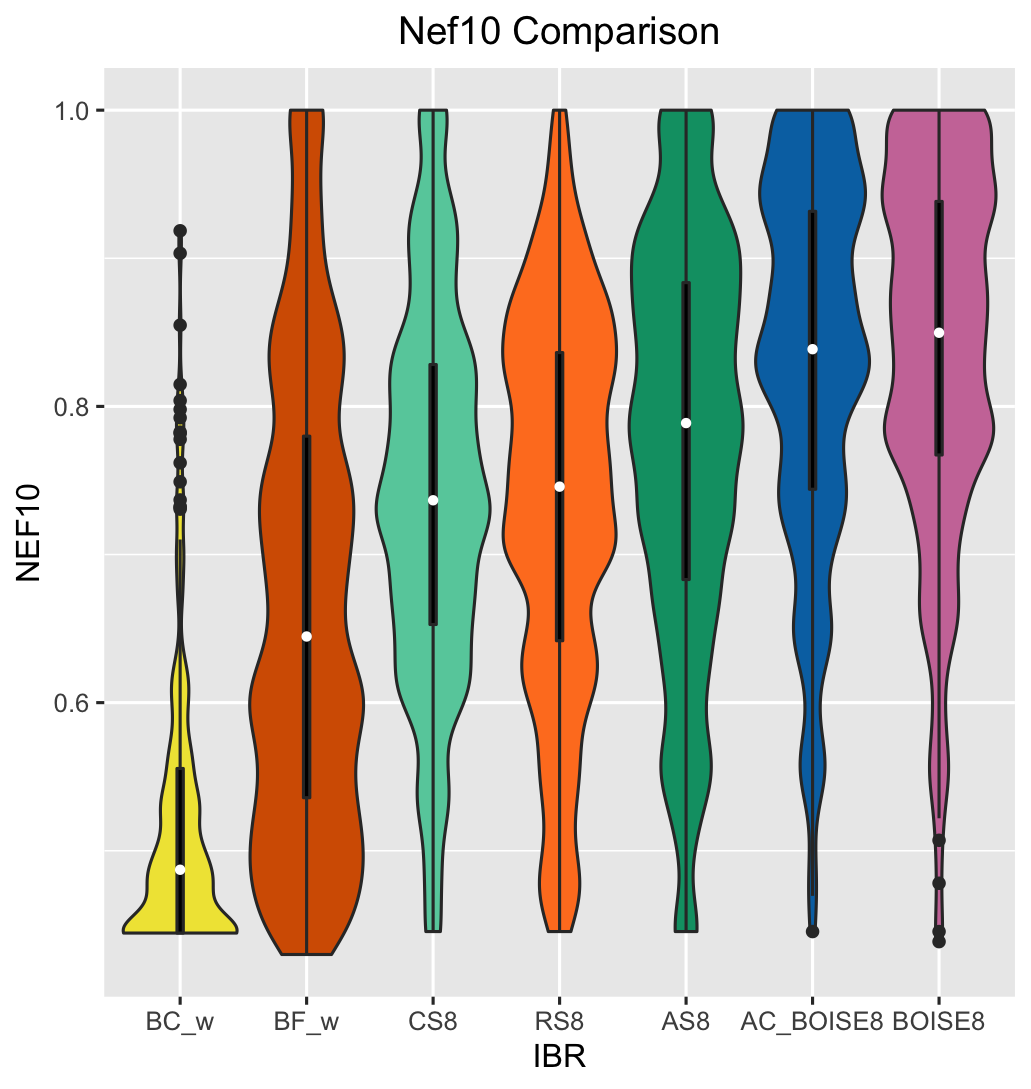
\includegraphics[width=5.0in]{pkis1_8_NEF10_AC.png}
\end{figure}

Similarly, from Figure 2 below we can see that Coding Selection (CS8) is the best method other than BOISE and Accelerated-BOISE under ROCAUC metric. By similar paired t-test, the mean difference between BOISE and CS is $0.0283$, with p-value $=3.73\times 10^{-6}$; the mean difference between AC-BOISE and CS is $0.0258$, with p-value $=3.035\times 10^{-5}$, and the difference between BOISE and AC-BOISE is $0.0024$, with p-value $=0.4578$.

\begin{figure}[!ht]
\caption{\label{fig:auc} 
{\bf Violin plot comparison of different methods under informer size $n_A =8$ with respect to compound ranking performance assessed by ROCAUC.} Each method is evaluated through leave one target out cross validation of PKIS1 targets. ROCAUC of 0.5 indicates a random guess, and ROCAUC of 1.0 represents ideal ranking with all active compounds prioritized above the inactives. The median and interquartile ranges are displayed as a white circle and black bars, respectively.} 
\centering
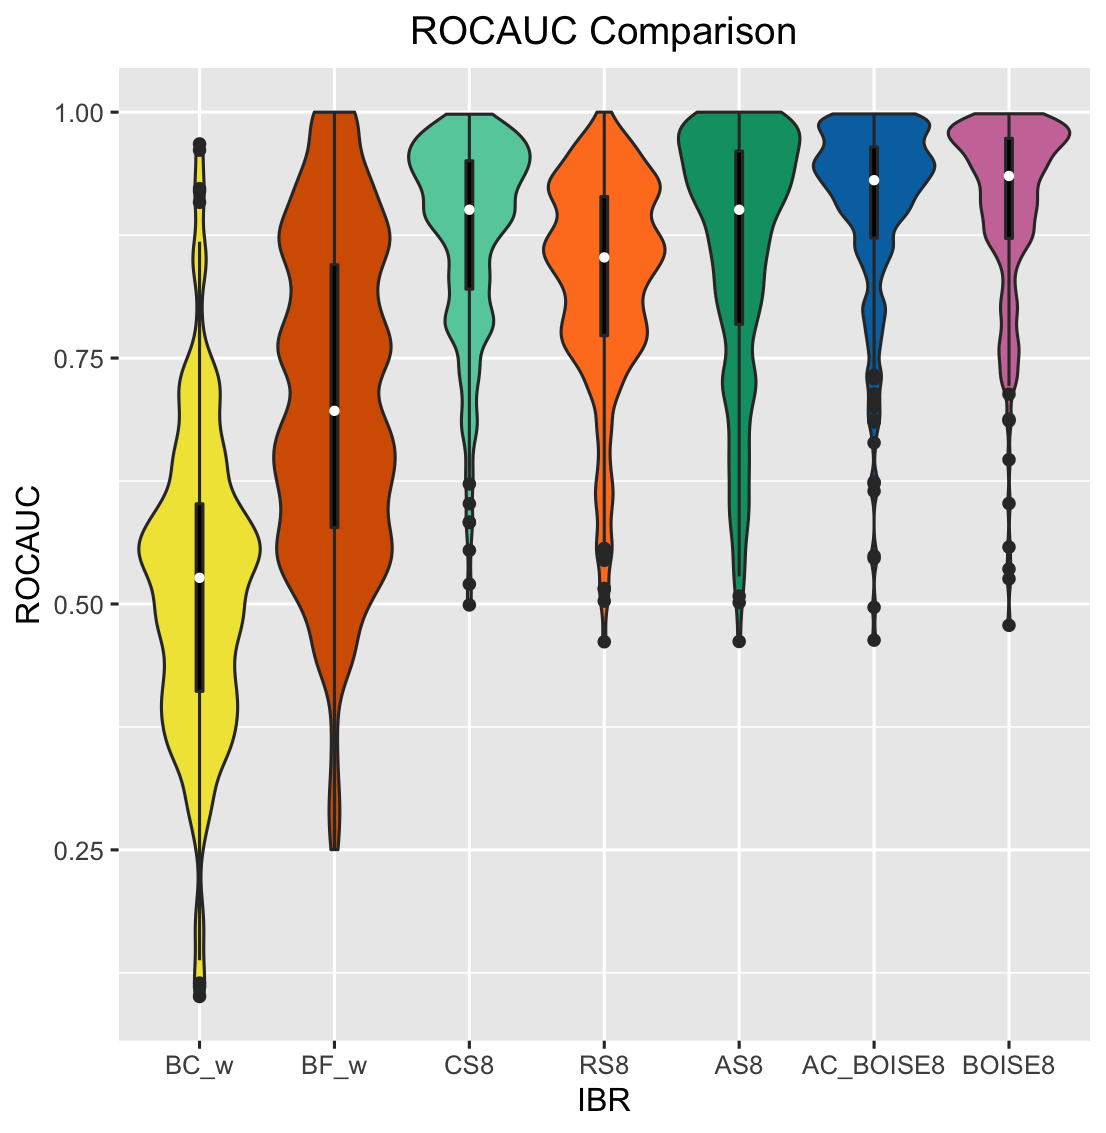
\includegraphics[width=5.0in]{pkis1_8_ROCAUC_AC.png}
\end{figure}

Same thing happens when we boost informer set size from $n_A = 8$ to $n_A = 16$. Since BOISE takes too much time for a leave-one-out cross validation under $n_A=16$, we can not afford it, instead we treat Accelerated-BOISE as a lower bound of BOISE performance as Figure 1 and Figure 2 tell us. Empirical results show that AC-BOISE is still significantly better than previous methods: Under NEF10 metric, Adaptive Selection (AS16) is the best method other than AC-BOISE and the paired t-test shows that their mean difference is $0.0415$ with p-value $=6.199\times 10^{-7}$;  Under ROCAUC metric, Regression Selection (RS16) is the best method other than AC-BOISE and the paired t-test shows that their mean difference is $0.0294$ with p-value $=1.303\times 10^{-4}$. More detailed results are summarized in following Figure 3 and Figure 4:
\begin{figure}[!ht]
\caption{\label{fig:nef2} 
{\bf Violin plot comparison of different methods under informer size $n_A =16$ with respect to compound ranking performance assessed by NEF10.}} 
\centering
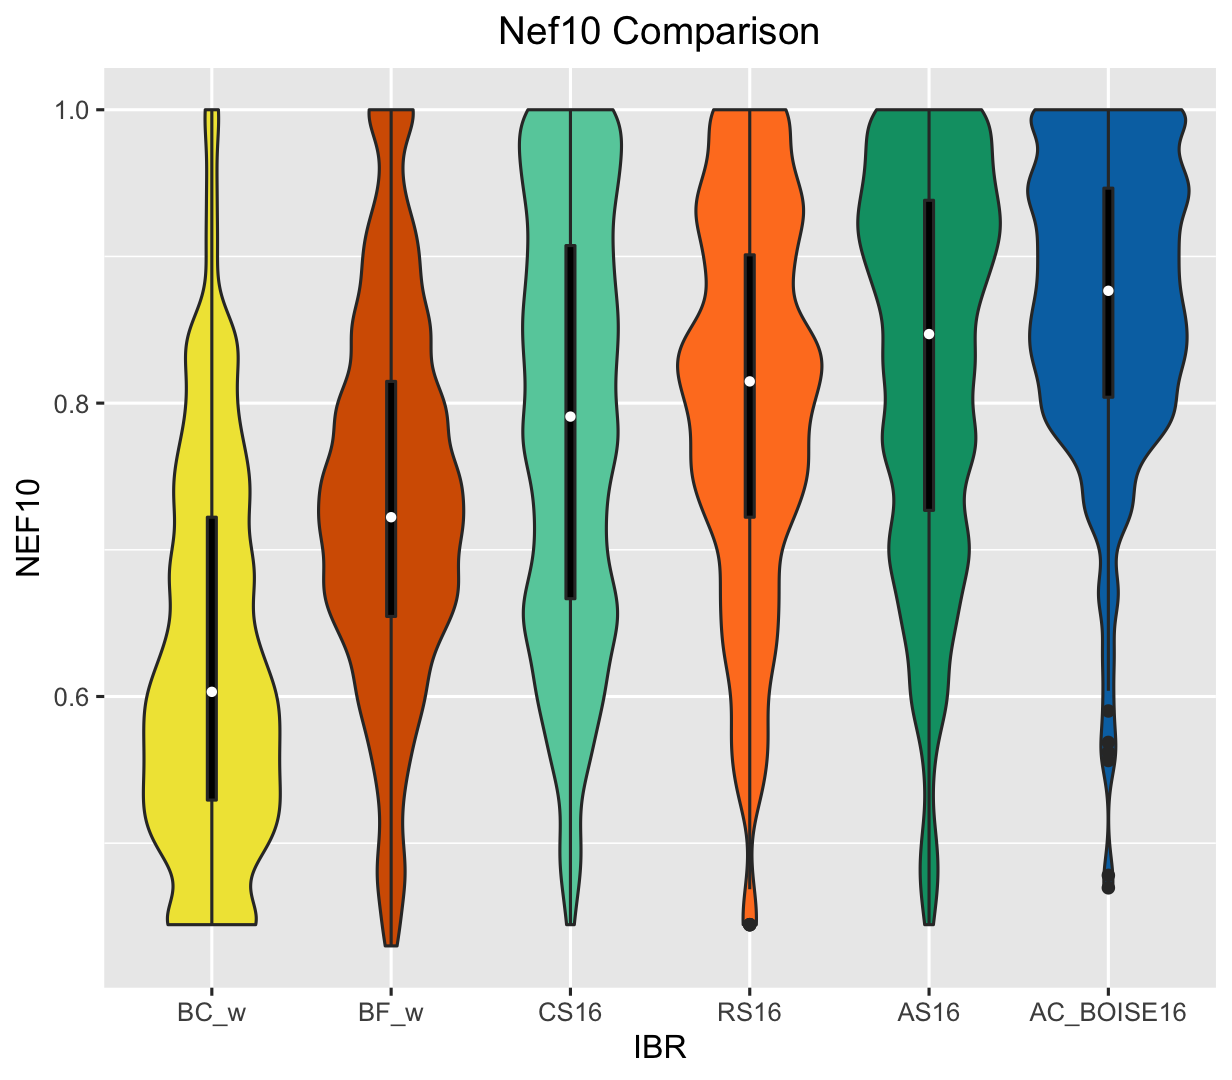
\includegraphics[width=5.0in]{pkis1_16_NEF10_AC.png}
\end{figure}

\begin{figure}[!ht]
\caption{\label{fig:auc2} 
{\bf Violin plot comparison of different methods under informer size $n_A =16$ with respect to compound ranking performance assessed by ROCAUC.}} 
\centering
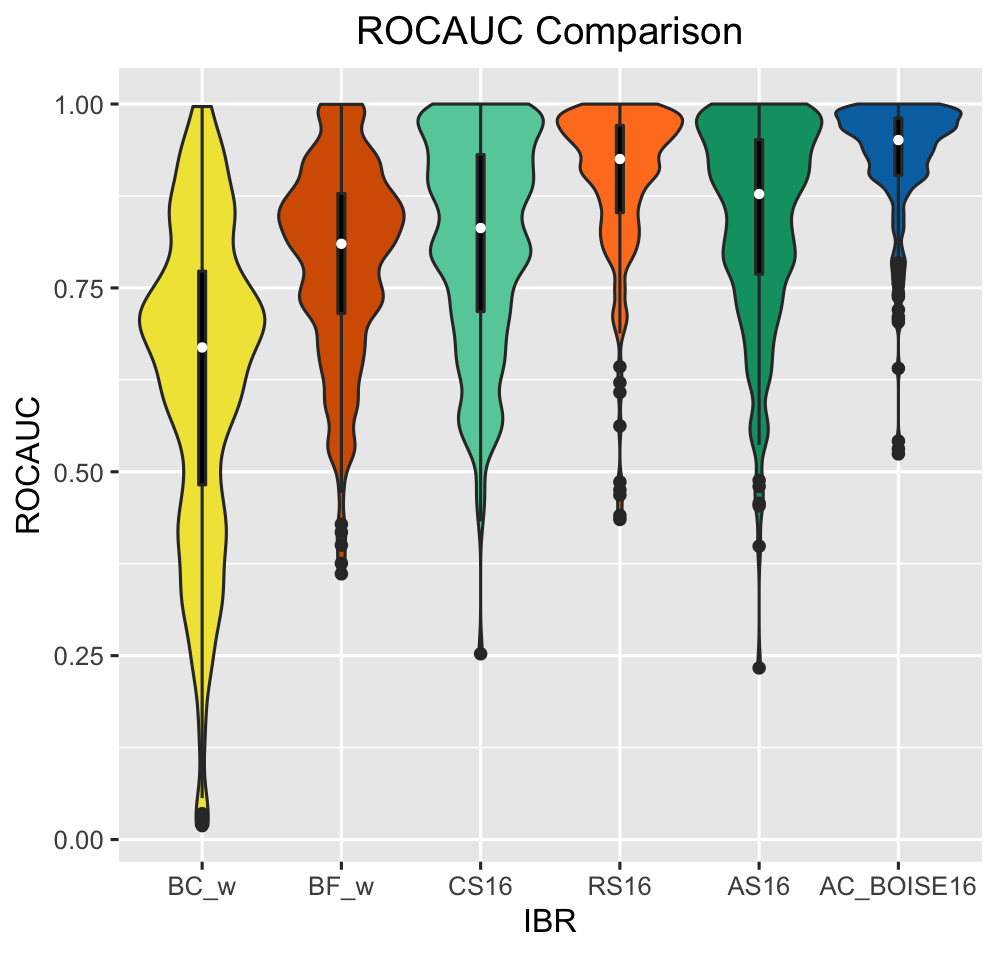
\includegraphics[width=5.0in]{pkis1_16_ROCAUC_AC.png}
\end{figure}

Moreover, there are some concerns about ROCAUC metric, saying that it will amplify the scores. To address these concerns, we include other well-known robust classification criteria like Matthews Correlation Coefficient (MCC) into our comparison. It turns out different criteria will do no harm to BOISE superiority. 

Recall that definition of MCC is:
\begin{eqnarray}
\label{eq:mcc}
MCC = \frac{TP\times TN-FP\times FN}{\sqrt{(TP+FP)(TP+FN)(TN+FP)(TN+FN)}}
\end{eqnarray}
where TP, FP, TN, FN come from confusion matrix. MCC takes value in $[-1,1]$, with MCC of $0$ indicates a random guess. Notice that MCC is for binary classification and we are doing ranking for compounds, we will just choose the best split point for our ranked compounds. From Figure 5 below, Adaptive Selection (AS8) is the best method other than AC-BOISE and BOISE under MCC. After paired t-test previously mentioned, the mean difference between AS8 and AC-BOISE is $0.0401$ with p-value $=2.839\times 10^{-5}$; and  mean difference between AS8 and BOISE is $0.0436$ with p-value $=3.722\times 10^{-6}$:

\begin{figure}[!ht]
\caption{\label{fig:auc2} 
{\bf Violin plot comparison of different methods under informer size $n_A =8$ with respect to compound ranking performance assessed by Matthews Correlation Coefficient (MCC).} Each method is evaluated through leave one target out cross validation of PKIS1 targets. MCC takes value in $[-1,1]$. MCC of $0$ indicates a random guess, and MCC of 1.0 represents ideal ranking with all active compounds prioritized above the inactives. The median and interquartile ranges are displayed as a white circle and black bars, respectively.} 
\centering
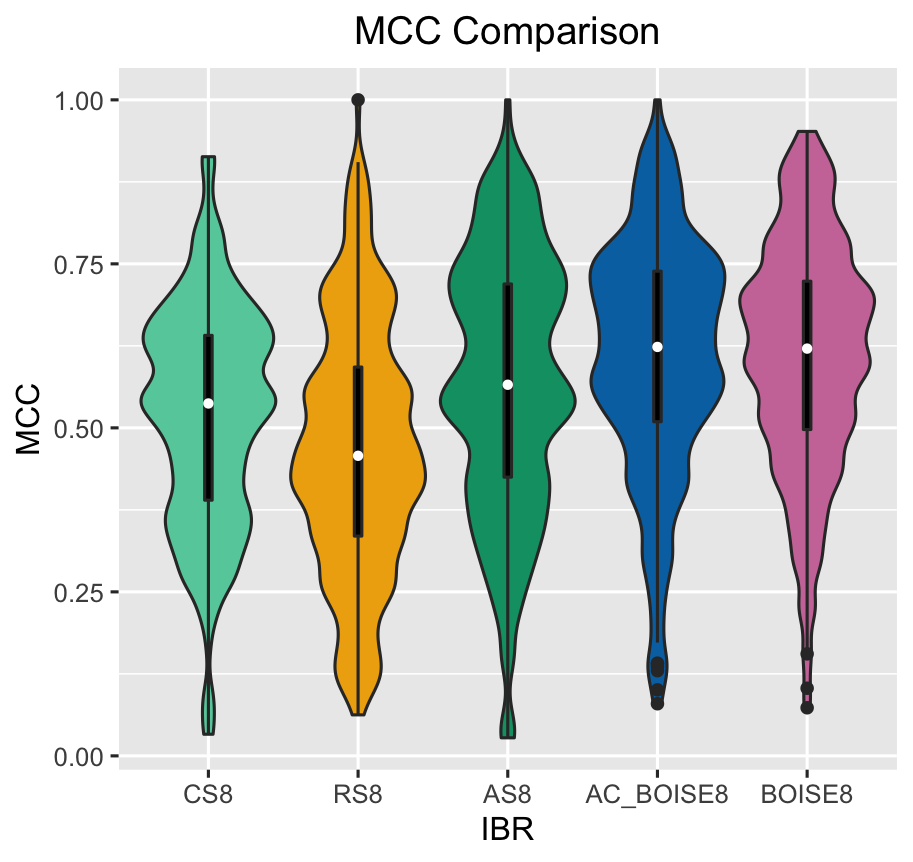
\includegraphics[width=5.0in]{pkis1_8_MCC.png}
\end{figure}

\subsection{GDSC Data Set}

\section{Discussion}

...on what to do next

...on connection to Bayesian adaptive design (e.g.
two-stage finite decision problems ; section 12.3.1 in 
Parmigiani and Inoue...connection to sequential clinical trials...

%\singlespacing
%\setlength\bibsep{0pt}
%\bibliographystyle{my-style}
%\bibliography{Placeholder}


\appendix 

\section{Proofs}
\subsection{Proof of Theorem 1}
\begin{proof}

Theorem 1 claims that for any given informer $A$ and intermediate data $x_A$, there exists a top-set rule 
\begin{eqnarray*}
T^*(A,x_A,x_0) = \left\{ j \in J: \; \sum_{k\in J} \mathbbm{1}(\hat \theta_{i^*k} > \hat \theta_{i^*j}) \leq n_T \right\}
\end{eqnarray*}
such that  $r(A,T) \geq r(A, T^*)$. In other words, given $A$ and $x_A$, the best top-set rule is to select top $n_T$ compounds with largest posterior mean. Recall the expression of Bayes risk: 
\begin{align*}
r(A, T) 
&= \int_{x_0} \int_{x_A} \int_\Theta  L\left( A, T \right) \, 
p(\theta, x_A,x_0)\, d\theta \, d x_A \, d x_0\\
&= \int_{x_0} \int_{x_A} \int_\Theta  L\left( A, T \right) \, 
p(\theta |x_A,x_0)p(x_A|x_0)p(x_0)\, d\theta \, d x_A \, d x_0
\end{align*}
To prove the Theorem, it is sufficient to show that for any possible fixed $x_A$, $x_0$, inequality 
\begin{eqnarray}
\label{eq:inequal1}
\int_\Theta  L\left( A, T \right) \, 
p(\theta |x_A,x_0) \, d\theta \geq \int_\Theta  L\left( A, T^* \right) \, 
p(\theta |x_A,x_0) \, d\theta
\end{eqnarray}holds, and this is obvious if we write loss function $L(A,T)$ explicitly:
\begin{align*}
\int_\Theta  L\left( A, T \right) \, p(\theta |x_A,x_0) \, d\theta &= \int_\Theta  ( n_T - \sum_{j\in T} \theta_{i^*j}) 
p(\theta |x_A,x_0) \, d\theta\\
&= n_T - \sum_{j\in T} \hat \theta_{i^*j}\\
&\geq n_T - \sum_{j\in T^*}  \hat \theta_{i^*j}\\
&= \int_\Theta  L\left( A, T^* \right) \, 
p(\theta |x_A,x_0) \, d\theta
\end{align*}
The equality comes from previous definition that $\hat \theta_{i^*j} = \mathbb E(\theta_{i^*j}|x_A,x_0)$.
\end{proof}

\subsection{Proof of Theorem 2}
\begin{proof}

When $x_0$ is given, we can write ${\mbox {\rm PEL}}_1(x_0,A)$ as ${\mbox {\rm PEL}}_1(A)$ for simplicity. To prove Theorem $2$ we only need to show that, for any set $A \subset J$, and any $k\notin A$, ${\mbox {\rm PEL}}_1(A\cup\{k\})\leq {\mbox {\rm PEL}}_1(A)$.

For simplicity of notation, we denote top set rule as 
$T_1^*(x_A,x_k) = T^*(A\cup\{k\}, x_{A\cup\{k\}}, x_0)$ and $T_2^*(x_A) = T^*(A, x_{A}, x_0)$. Recall that:
\begin{eqnarray*}
    {\mbox {\rm PEL}}_1(A\cup\{k\})= \int_{x_{A}}\int_{x_k} p\left( x_{A},x_k | x_0 \right) 
\left[ \sum_{j \in  T_1^*(x_A,x_k)}  1 - \mathbb{E} (\theta_{i^*,j} \, |\, x_0,x_A,x_k) \right]dx_A dx_k
\end{eqnarray*}

From the fact that $T_1^*(x_A,x_k)$ is the Bayes rule when $A\cup\{k\}$, $x_{A\cup\{k\}}$ and $x_0$ are given, it should be no worse than $T_2^*(x_A)$ with regard to posterior expected loss, and hence we have:

\begin{align*}
&\int_{x_{A}}\int_{x_k} p\left( x_{A},x_k | x_0 \right)
\left[ \sum_{j \in  T_1^*(x_A,x_k)}  1 - \mathbb{E} (\theta_{i^*,j} \, |\, x_0,x_A,x_k) \right]\\ 
&\leq 
\int_{x_{A}}\int_{x_k} p\left( x_{A},x_k | x_0 \right)
\left[ \sum_{j \in  T_2^*(x_A)}  1 - \mathbb{E} (\theta_{i^*,j} \, |\, x_0,x_A,x_k) \right]
\end{align*}

Notice that in our model, $x_A \indep x_k \, | \, \theta_{i^*}$ and $\theta_{i^*A}\indep \theta_{i^*k}\, | \, x_0$. So we have $x_A\indep x_k\,|\, x_0$, and hence:

\begin{align*}
&\int_{x_{A}}\int_{x_k} p\left( x_{A},x_k | x_0 \right)
\left[ \sum_{j \in  T_2^*(x_A)}  1 - \mathbb{E} (\theta_{i^*,j} \, |\, x_0,x_A,x_k) \right]\\
    &= \int_{x_{A}}p\left(x_A|x_0\right)\sum_{j \in  T_2^*(x_A)}\left[\int_{x_k}p(x_k|x_0)\left(1-\mathbb{E} (\theta_{i^*,j} \, |\, x_0,x_A,x_k)\right)\right]\\
&= \int_{x_{A}}p\left(x_A|x_0\right) \sum_{j \in  T_2^*(x_A)}\left[  1 - \mathbb{E} (\theta_{i^*,j} \, |\, x_0,x_A) \right].
\end{align*}


The first equality is because $T_2^*(x_A)$ is a function only of $x_A$. 

This implies ${\mbox {\rm PEL}}_1(A\cup\{k\})\leq {\mbox {\rm PEL}}_1(A)$, and the equality holds if and only if $T_1^*(x_A,x_k) = T_2^*(x_A)$, which means top sets are the same for any possible outcomes $x_A$ and $x_k$. 

\end{proof}

\subsection{Frequent hitters rule}

**Peng inserts proof about this **

\textbf{Proposition for new settings}

Under our new settings:
\begin{eqnarray*}
&x_{i,j}|\beta_j \sim_{ind} {\rm Bernoulli}(\beta_j);\\
&\beta_j \sim_{i.i.d} {\rm Beta}(a,b)
\end{eqnarray*}

Let $s_k = \sum_{i = 1}^n x_{ik}$ be column sums. We can assume that $s_1 \leq s_2 \leq~...~\leq s_m$.

Since it's conjugate prior, we have the posterior distribution:
\begin{eqnarray*}
\beta_j | x_0 \sim {\rm Beta}(a + s_j, b + n - s_j)
\end{eqnarray*}
\begin{equation}
\beta_j|x_0,x_A \sim \left\{
\begin{aligned}
&{\rm Beta}(a+s_j, b+n-s_j),{\rm if}~j\notin A,\\
&{\rm Beta}(a+s_j+x_j^*, b+n+1-s_j-x_j^*),{\rm if}~j\in A,\\
\end{aligned}
\right.
\end{equation}

and the posterior expectation:
\begin{equation}
E(\beta_j|x_0,x_A) = \left\{
\begin{aligned}
&(a + s_j)/(a + b + n),{\rm if}~j\notin A,\\
&(a + s_j + x_j^*)/(a + b + n +1),{\rm if}~j\in A,\\
\end{aligned}
\right.
\end{equation}

We first prove a general proposition:

\begin{proposition}
Given $n_A$, $n_T$ and the setting above, if for different informer sets $A_1$ and $A_2$, for any $0-1$ sequence $\nu$, $\hat{T}(A_1, x_{A_1} = \nu) = \hat{T}(A_2,x_{A_2} = \nu) \equiv T$, i.e. Top set is constant w.r.t. any results of two different informer sets. Then ${\rm PEL}_1(x_0, A_1) = {\rm PEL}_1(x_0, A_2)$.
\end{proposition}

\begin{proof}
Let $\Omega = \{$All the 0-1 sequences of length $n_A \}$ be the sample space of $x_{A_1}$. Then $P(x_{A_1}|x_0)$ is a probability measure on $\Omega$. By applying Fubini theorem several times, we have: 
\begin{align*}
    n_A - {\rm PEL}_1(x_0, A_1) &= \int_\Omega P(x_{A_1} = s|x_0)\sum_{j\in T} E(\beta_j|x_0, x_{A_1} = s) ~{\rm d}s\\
    &= \sum_{j\in T} \int_\Omega \int_{[0,1]} \beta_j \times \frac{P(\beta_j,x_0,x_{A_1}=s )}{P(x_0,x_{A_1} = s)}\times \frac{P(x_{A_1} = s, x_0)}{P(x_0)}~{\rm d}\beta_j~{\rm d}s\\
    &= \sum_{j \in T} \int_{[0,1]}\int_\Omega \beta_j P(\beta_j, x_{A_1} = s|x_0) ~{\rm d}s~{\rm d}\beta_j\\
    &= \sum_{j\in T}E(\beta_j|x_0)
\end{align*}

Since the value of ${\rm PEL}_1(x_0,A_1)$ has nothing to do with informer set $A_1$, ${\rm PEL}_1(x_0, A) \equiv Const.$ for any informer sets.
\end{proof}

Consider now there are no ties in $s_j$'s, we will show that ${\rm PEL}_1(x_0, A)$ is constant risk for any $A$.

Notice that when $s_1 < s_2 < s_3 <...<s_m$, we can rewrite them as $s_i + 1\leq s_{i+1}$.

From inequalities 
$$
\frac{a+s_i}{a+b+n} < \frac{a+s_i+1}{a+b+n+1} \leq \frac{a+s_{i+1}}{a+b+n+1}
$$

and 
$$
\frac{a+s_i}{a+b+n} <
\frac{a+s_i+1}{a+b+n+1} \leq \frac{a+s_{i+1}}{a+b+n}
$$

and 
$$
\frac{a+s_i+1}{a+b+n+1} < \frac{a+s_i+1}{a+b+n} \leq \frac{a+s_{i+1}}{a+b+n}
$$

We have:
$$
E(\beta_i|x_0, x_i^* = 0, x_k^* = 1) \geq
E(\beta_k|x_0,x_i^* = 0, x_k^* = 1), {\rm for}~k < i;
$$

and
$$
E(\beta_i|x_0, x_j^*, x_k^* = 1) > E(\beta_k|x_0,x_j^* = 1, x_k^* = 1), {\rm for}~k < i, j \neq i,k.
$$

This means: When there is no ties, $E(\beta_i|x_0, x_A) \geq E(\beta_k|x_0, x_A)$ for any $k < i$ and $x_A$. Therefore, we will choose a constant Top set $T = \{m-n_T+1,~...,~m-1,~m\}$ w.r.t any informer set $A$ and any results of $x_A$. 

From our previous Proposition, when there is no ties, Top set is constant w.r.t. any results of different informer sets, and hence ${\rm PEL}_1(x_0, A)\equiv Const.$ for any A. 

\textbf{Here is an counter-example}

We now show that: when $n_A = 1$, $n_T = 2$, and $s_m > s_{m-1} = s_{m-2}$, $A^* = \{m-1\}$ is better than the Frequent Hitters Rule $\hat{A} = \{m\}$ in our framework.

First calculate $P(x_A|x_0)$:
\begin{align*}
    P(x_A|x_0) &= \frac{\int_\beta P(x_A, x_0|\beta_1,...,\beta_m)P(\beta_1,...,\beta_m){\rm d}\beta}{P(x_0)}\\
    &= \frac{\int_\beta P(x_A|\beta_1,...,\beta_m)P(x_0,\beta_1,...,\beta_m){\rm d}\beta}{P(x_0)}\\
    &= \int_\beta P(x_A|\beta_1,...,\beta_m)P(\beta_1,...,\beta_m|x_0){\rm d}\beta\\
    &= \int_{\beta_A} P(x_A|\beta_A)P(\beta_A|x_0){\rm d}\beta_A\\
    &= \int_{\beta_A} \frac{\Gamma(a+b+n)}{\Gamma(a+s_A)\Gamma(b+n-s_A)}\beta_A^{x_A}(1 - \beta_A)^{1-x_A}\beta_A^{a+s_A - 1}(1-\beta_A)^{b+n-s_A-1}{\rm d}\beta_A\\
    &= \frac{1}{a+b+n}\times\frac{\Gamma(a+s_A+x_A)\Gamma(b+n+1-x_A-s_A))}{\Gamma(a+s_A)\Gamma(b+n-s_A)}
\end{align*}

Next calculate ${\rm PEL}_1(x_0,A)$:

Recall $\hat{A} = \{m\}$ and $A^* = \{m-1\}$. Notice that whenever $x_{\hat{A}} = 0~ {\rm or} ~1$, $\hat{T}^*(x_0,x_{\hat{A}}) = \{m-1,m\}$. 

\begin{align*}
    n_T - {\rm PEL}_1(x_0, \hat{A}) &= P(x_m^* = 1|x_0)(E(\beta_m|x_0,x_m^* = 1) + E(\beta_{m-1}|x_0, x_m^* = 1)) +\\ &~~~~P(x_m^* = 0|x_0)(E(\beta_m|x_0,x_m^* = 0) + E(\beta_{m-1}|x_0, x_m^* = 0))\\
    &= \frac{a+s_m}{a+b+n}\times (\frac{a+s_m+1}{a+b+n+1} + \frac{a+s_{m-1}}{a+b+n})+\\ &~~~~\frac{b+n-s_m}{a+b+n}\times(\frac{a+s_m}{a+b+n+1} + \frac{a+s_{m-1}}{a+b+n})\\
    &= \frac{(a + s_m) + (a+s_{m-1})}{a+b+n}
\end{align*}

and when $x_{A^*} = 1$, $\hat{T}^*(x_0,x_{A^*}) = \{m-1,m\}$; When $x_{A^*} = 0$, since $$
E(\beta_{m-1}|x_0,x_{m-1}^* = 0) < E(\beta_{m-2}|x_0,x_{m-1}^* = 0)<E(\beta_m|x_0,x_{m-1}^* = 0)
$$ 

we have $\hat{T}^*(x_0,x_{A^*}) = \{m,m-2\}$.

\begin{align*}
    n_T - {\rm PEL}_1(x_0, A^*) &= P(x_{m-1}^* = 1|x_0)(E(\beta_m|x_0,x_{m-1}^* = 1) + E(\beta_{m-1}|x_0, x_{m-1}^* = 1)) +\\ &~~~~P(x_{m-1}^* = 0|x_0)(E(\beta_m|x_0,x_{m-1}^* = 0) + E(\beta_{m-2}|x_0, x_{m-1}^* = 0))\\
    &= \frac{a+s_{m-1}}{a+b+n}\times (\frac{a+s_{m-1}+1}{a+b+n+1} + \frac{a+s_m}{a+b+n})+\\ &~~~~\frac{b+n-s_{m-1}}{a+b+n}\times(\frac{a+s_{m-2}}{a+b+n} + \frac{a+s_m}{a+b+n})\\
    &= \frac{a + s_m}{a+b+n} + \frac{a+s_{m-1}}{a+b+n}(\frac{a+s_{m-1}+ 1}{a+b+n+1} + \frac{b+n-s_{m-1}}{a+b+n})
\end{align*}

Since:
$$
\frac{a+s_{m-1}+1}{a+b+n+1} > \frac{a+s_{m-1}}{a+b+n}.
$$

We have 
$n_T - {\rm PEL}_1(x_0, \hat{A}) <n_T - {\rm PEL}_1(x_0, A^*)$, 
so $\hat{A}$ is not the Bayes Rule.

\textbf{Intuition:} From analysis above, it seems like we should first choose the "Transition Part" as informer set instead of the "Most-possible Part". For example, if $n_A = 2$, $n_T = 10$, $s_1 \geq s2 \geq ~...~\geq s_m$ defined same as before, than we should choose $\{9, 10\}$, not $\{1, 2\}$.

\onehalfspacing

%\section*{Tables} \label{sec:tab}
%\addcontentsline{toc}{section}{Tables}



%\clearpage

%\section*{Figures} \label{sec:fig}
%\addcontentsline{toc}{section}{Figures}

%\begin{figure}[hp]
%  \centering
%  \includegraphics[width=.6\textwidth]{../fig/placeholder.pdf}
%  \caption{Placeholder}
%  \label{fig:placeholder}
%\end{figure}



\section*{References}

\begin{list}{}{}
\item Berger, J.O. (1985). {\em Statistical decision theory and Bayesian analysis}. 2nd ed. Springer-Verlag, New York.

\item Carpenter, B., Gelman, A., Hoffman, M.D., Lee, D., Goodrich, B., Betancourt, M., Brubaker, M., Guo, J., Li, P. and Riddell, A., 2017. Stan: A probabilistic programming language. {\em Journal of statistical software}, 76(1).

\item Henderson, N. (2015). {\em Methods for Ranking and Selection in Large-Scale Inference.} PhD Thesis,
University of Wisconsin, Madison.

\item Li, H. and Hong, F., (2001). Cluster-Rasch models for microarray gene expression data. {\em Genome biology}, 2(8), pp.research0031-1.

\item Parmigiani, G. and Inoue, L. (2009). {\em Decision theory: principles and approaches} (Vol. 812). John Wiley \& Sons.

\item Reker, D and Schneider, G (2015). Active-learning 
strategies in computer-assisted drug design. **

\item Robert, C. (2007). {\em The Bayesian choice: from decision-theoretic foundations to computational implementation.} Springer Science \& Business Media.

\item Sliwoski, G., Kothiwale, S., Meiler, J. and Lowe, E.W. (2014). Computational methods in drug discovery. {\em Pharmacological reviews}, 66(1), pp.334-395.

\item  Zhang, H.,   Ericksen, S.S.,  Lee, C.,  Ananiev, G.E., Wlodarchak, N.,  Mitchell, J.C.,  Gitter, A.,  Wright, S.J., Hoffmann, F.M.,  Wildman, S.A., and 
Newton, M.A. (2019). Predicting kinase inhibitors using bioactivity matrix derived informer sets.
\verb+bioarXiv+

\end{list}



\end{document}